%: ----------------------- sigex file header -----------------------
\chapter{Chameleons}
\label{sec:chameleons}

% the code below specifies where the figures are stored
\ifpdf
    \graphicspath{{chameleons}{chameleons/figures/PDF/}{chameleons/figures/}}
\else
    \graphicspath{{chameleons/figures/EPS/}{chameleons/figures/}}
\fi

% ----------------------------------------------------------------------
% ----------------------- chameleons content -------------------------
% ----------------------------------------------------------------------

The current global best fit value for  $\Delta m^{2}_{21}$ and
$\theta_{12}$ comes
primarily from a combined fit to solar neutrino data from SNO
and SuperK and Borexino, and reactor neutrino data from KamLAND\@.
These fits have produced the values
\begin{equation}
    \Delta m^{2}_{21} = 7.39^{+0.21}_{-0.21}\times10^5 \text{eV}^{2}
\end{equation}
\begin{equation}
    \sin^2\theta_{12} = 0.310^{+0.013}_{-0.012}\text{.}
\end{equation}
However, KamLAND has much better sensitivity to $\Delta m^{2}_{21}$
than the combined SNO and SuperK result, so the best fit value for
$\Delta m^{2}_{21}$ comes almost exclusively from the KamLAND
reactor neutrino measurements.

\begin{figure}[htbp]
    \centering
    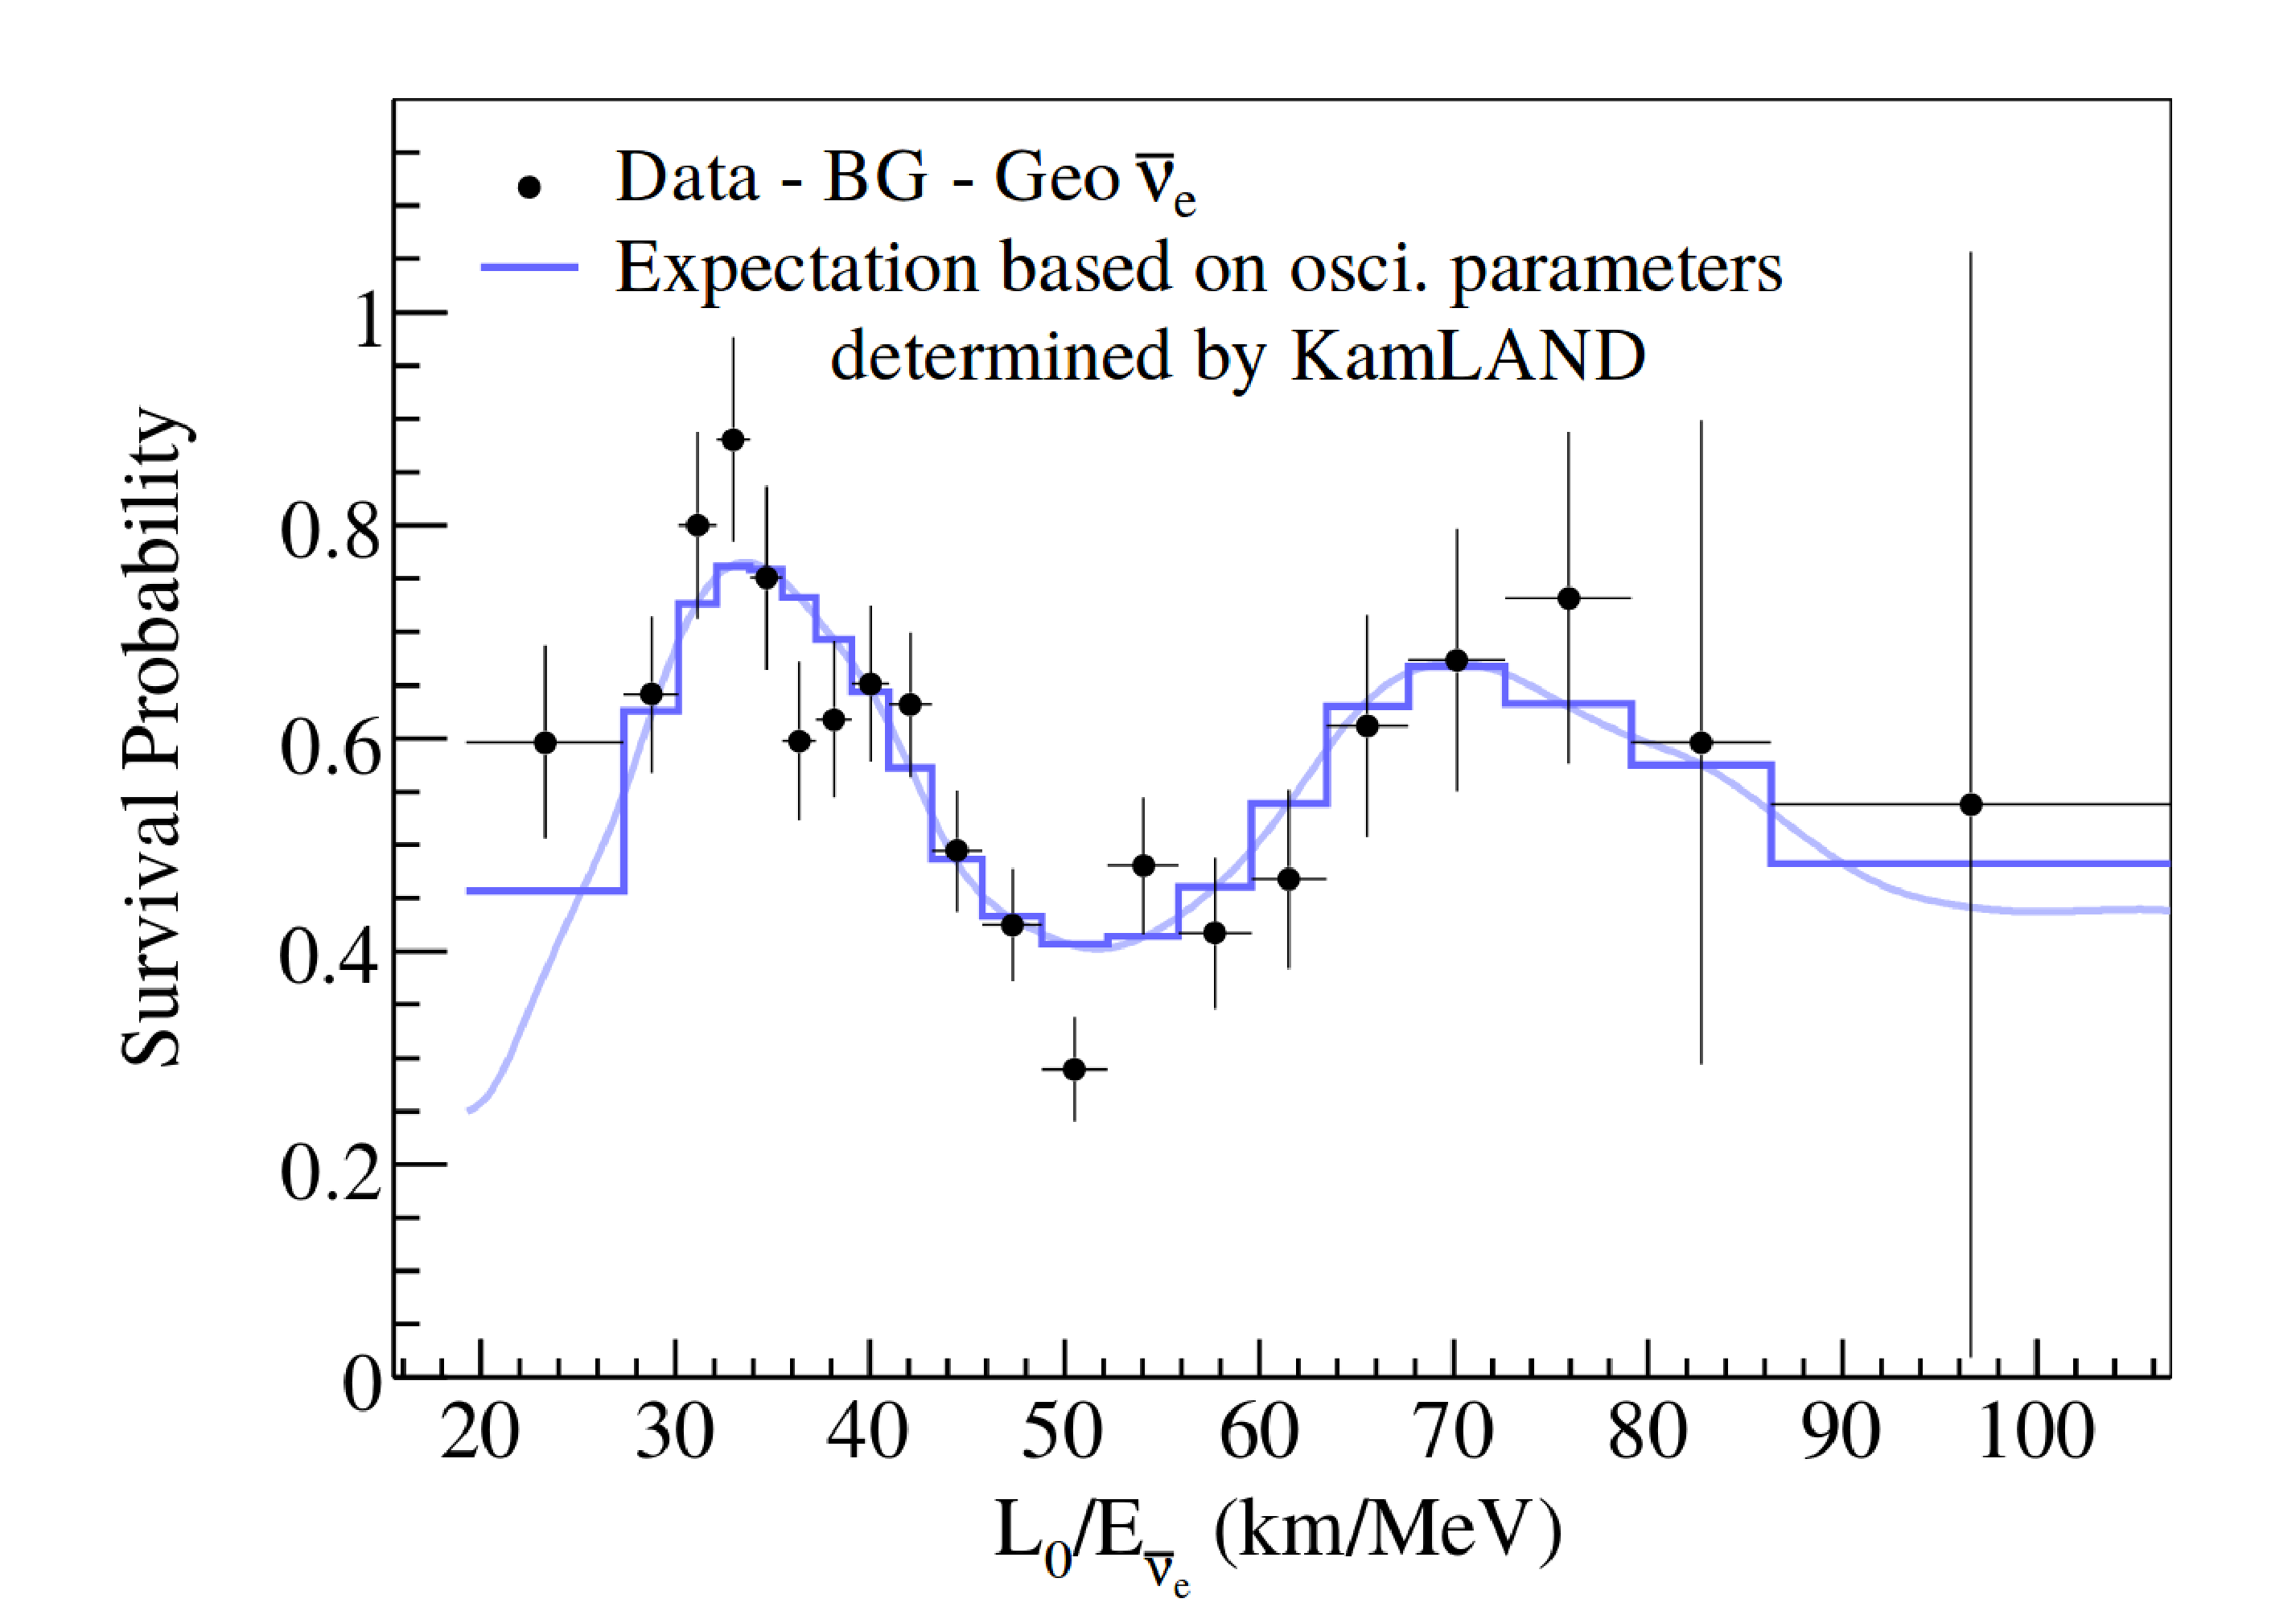
\includegraphics[width=\textwidth]{kamland_oscillation}
    \caption[]{}
    \label{fig:kamland_oscillation}
\end{figure}
The KamLAND measurement is discussed briefly in Sec~\ref{sec:kamland}.
The precision of their measurement comes from the fact that $\Delta m^{2}_{21}$
adjusts the ``wavelength'' in energy of oscillations in their observed
reactor neutrino spectrum.
Figure~\ref{fig:kamland_oscillation} shows KamLAND's observed oscillation
spectrum and best fit.

\begin{figure}[htbp]
    \centering
    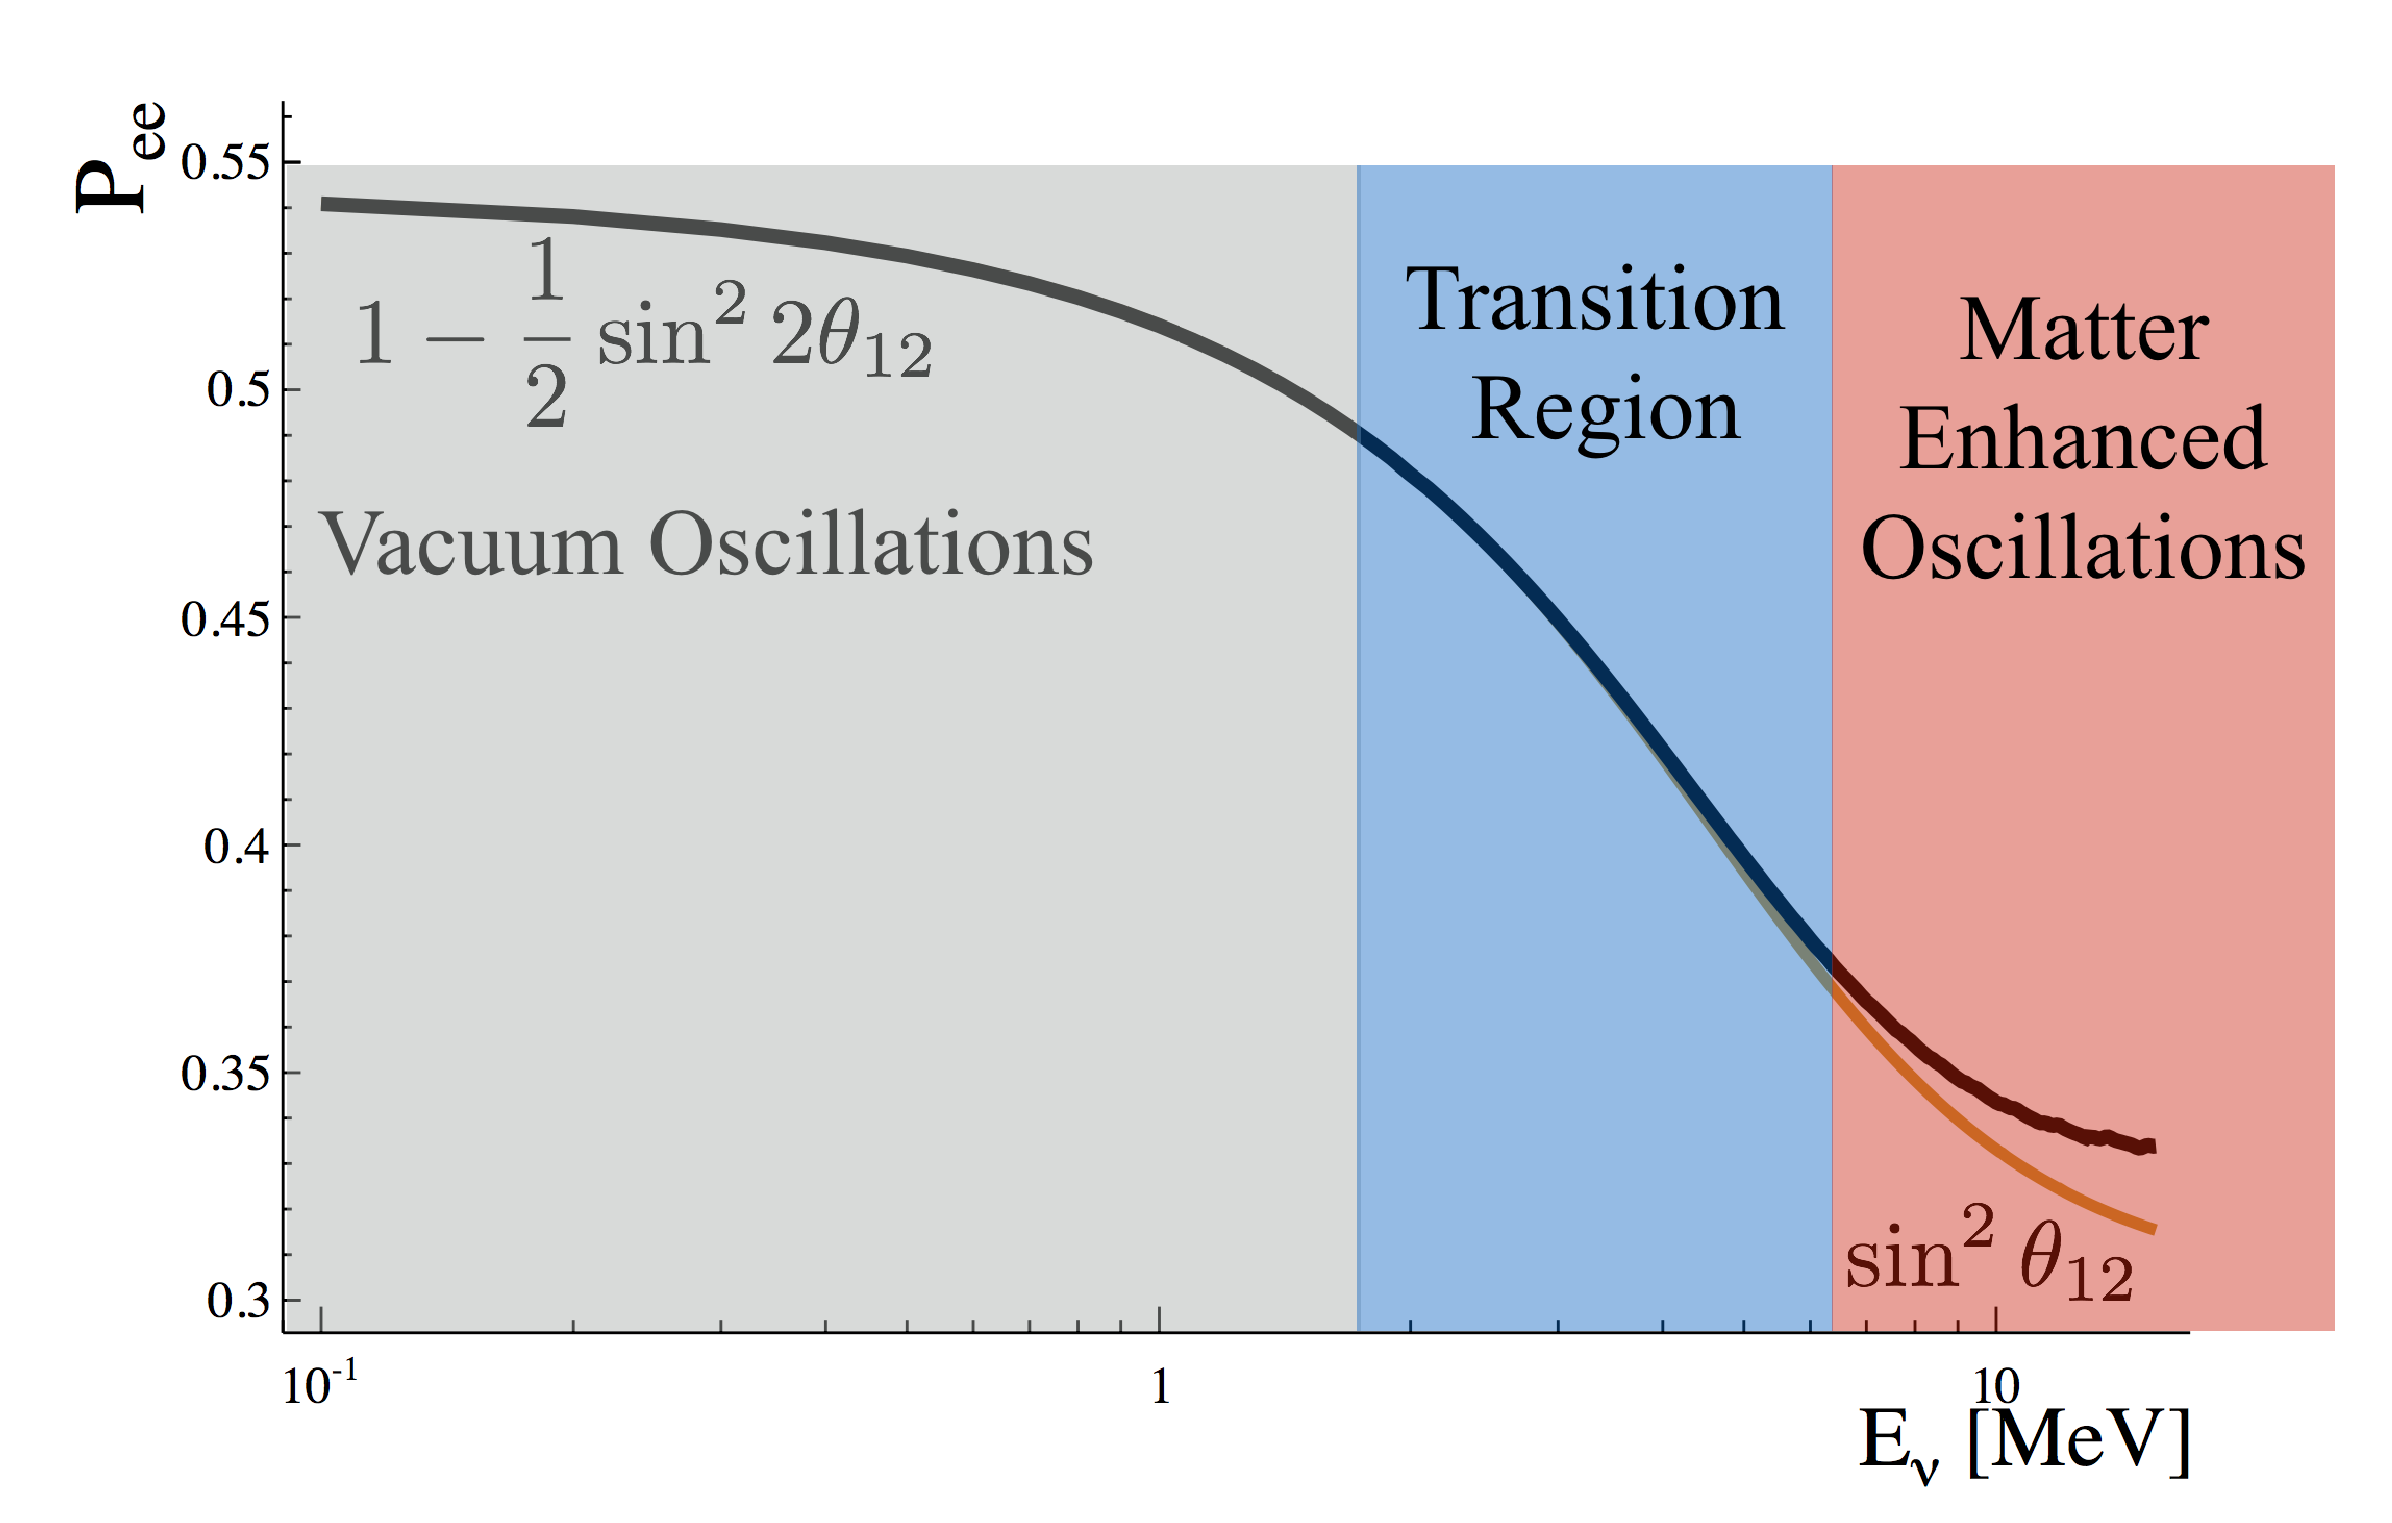
\includegraphics[width=\textwidth]{labelled_survival_probability}
    \caption[]{}
    \label{fig:labelled_pee}
\end{figure}

Figure~\ref{fig:labelled_pee} shows the solar survival probability,
with labelled features.
The transition region is where the survival probability changes from
being very close to the vacuum survival probability at low energies,
to being dominated by matter effects at the higher energies.
The width of the transition region comes from the radial production
distribution of solar neutrinos in the sun;
Neutrinos at energies high enough to experience significant matter
effects in the sun, may or may not be in an area of the Sun with sufficient
electron density to provide a strong matter effect.
The reason the solar neutrino experiments are relatively insensitive
to $\Delta m^{2}_{21}$ is because the only effect it has on the
solar neutrino survival probability is to shift the energy
of the MSW-transition region, a smaller value for $\Delta m^{2}_{21}$ results
a lower energy transition region.
At energies in the middle of transition region, you'll observe approximately
as many neutrinos that never experience significant matter effects as neutrinos
that did.
For experiments, this means sensitivity to $\Delta m^{2}_{21}$ comes
primarily from their ability to measure the survival probability in the
transition region compared to in the vacuum or matter dominate regions.

In principal this means solar neutrino experiments should be very sensitive
to $\Delta m^{2}_{21}$, a good measurement of neutrino oscillation probability
in the transition region is all that is required.
However, the Sun does not provide a optimal source of neutrinos at energies
in the transition region.
The $\ce{^{8}B}$ and $hep$ reactions provide neutrinos at energies across the
entirety of the transition region, but the flux of each of those sources is
very small, especially at energies between $1-3$\,MeV\@;
At energies below $15$\,MeV the $\ce{^{8}B}$ flux is dominant over the $hep$
flux.

The challenge of detecting relatively low energy, low flux $\ce{^{8}B}$ neutrinos
is made more difficult by the fact that at those energies radioactive backgrounds
are dominant in water Cherenkov detectors.
Most notably backgrounds from $\ce{^{214}Bi}$ and $\ce{^{208}Tl}$ contamination
which each provide a $\beta$ with a spectrum that respectively have a decay
Q-value of $3.2$\,MeV and $5.0$\,MeV.
These background render $\ce{^{8}B}$ neutrino measurements in the transition
region nearly impossible for water Cherenkov detectors.
For a liquid scintillator detector, target volume can be purified to a greater
degree than a water detector, which mitigates
background contamination somewhat.
However, scintillator detectors cannot in general reconstruct the direction
of the neutrino, and so solar neutrinos cannot be identified against backgrounds.
And so even with higher radio-purity, at energies below approximately $3\,MeV$,
the $^{8}B$ solar neutrino flux is extremely difficult to measure for scintillator detectors..

Beyond the difficulty of measuring solar neutrinos at energies in the transition
region, is the fact that the most common way to measure solar neutrinos for
water Cherenkov or scintillator detectors
is through the electron elastic scattering interaction.
And as discussed in Sec~\ref{sec:esxsec} the energy of the observable
scattered electron is weakly correlated with the energy of the incoming neutrino.
And so even if a measurement of $\ce{^{8}B}$ solar neutrino interaction rate at low energies was
made, that interaction rate would include contributions from $\ce{^{8}B}$ neutrinos
from the observed energy up to the end-point energy.
Meaning any measurement performed in the transition region will contain many
more interactions from neutrinos with energy above the transition region than within
the transition region.
This means any measurement will require a very high statistics dataset to make
a good measurement of the solar neutrino survival probability in the transition
region.

Despite these difficulties the $\ce{^{8}B}$ survival probability has been measured
down to $3.5\,MeV$, though uncertainties at the lower energies are significant.
These measurements come from the SuperK elastic scattering measurements~\citep{superk4}, combined
with the three-phase SNO elastic scattering, charged current and neutral current measurements
~\citep{sno_combined}.
The SNO measurement provides the strongest constraints on the full, all-flavor, $\ce{^{8}B}$
flux, and the SuperK measurement provides the strongest constraints on the
flavor sensitive ``elastic-scattering'' flux.
So far these experiments have not seen strong evidence for any
upward transition in the survival probability.
Figure~\ref{fig:es_b8_measurement} shows the SNO measurement
and the combined SNO + SuperK  measurement

\begin{figure}[htbp]
    \centering
    \begin{subfigure}[b]{0.38\textwidth}
        \centering
    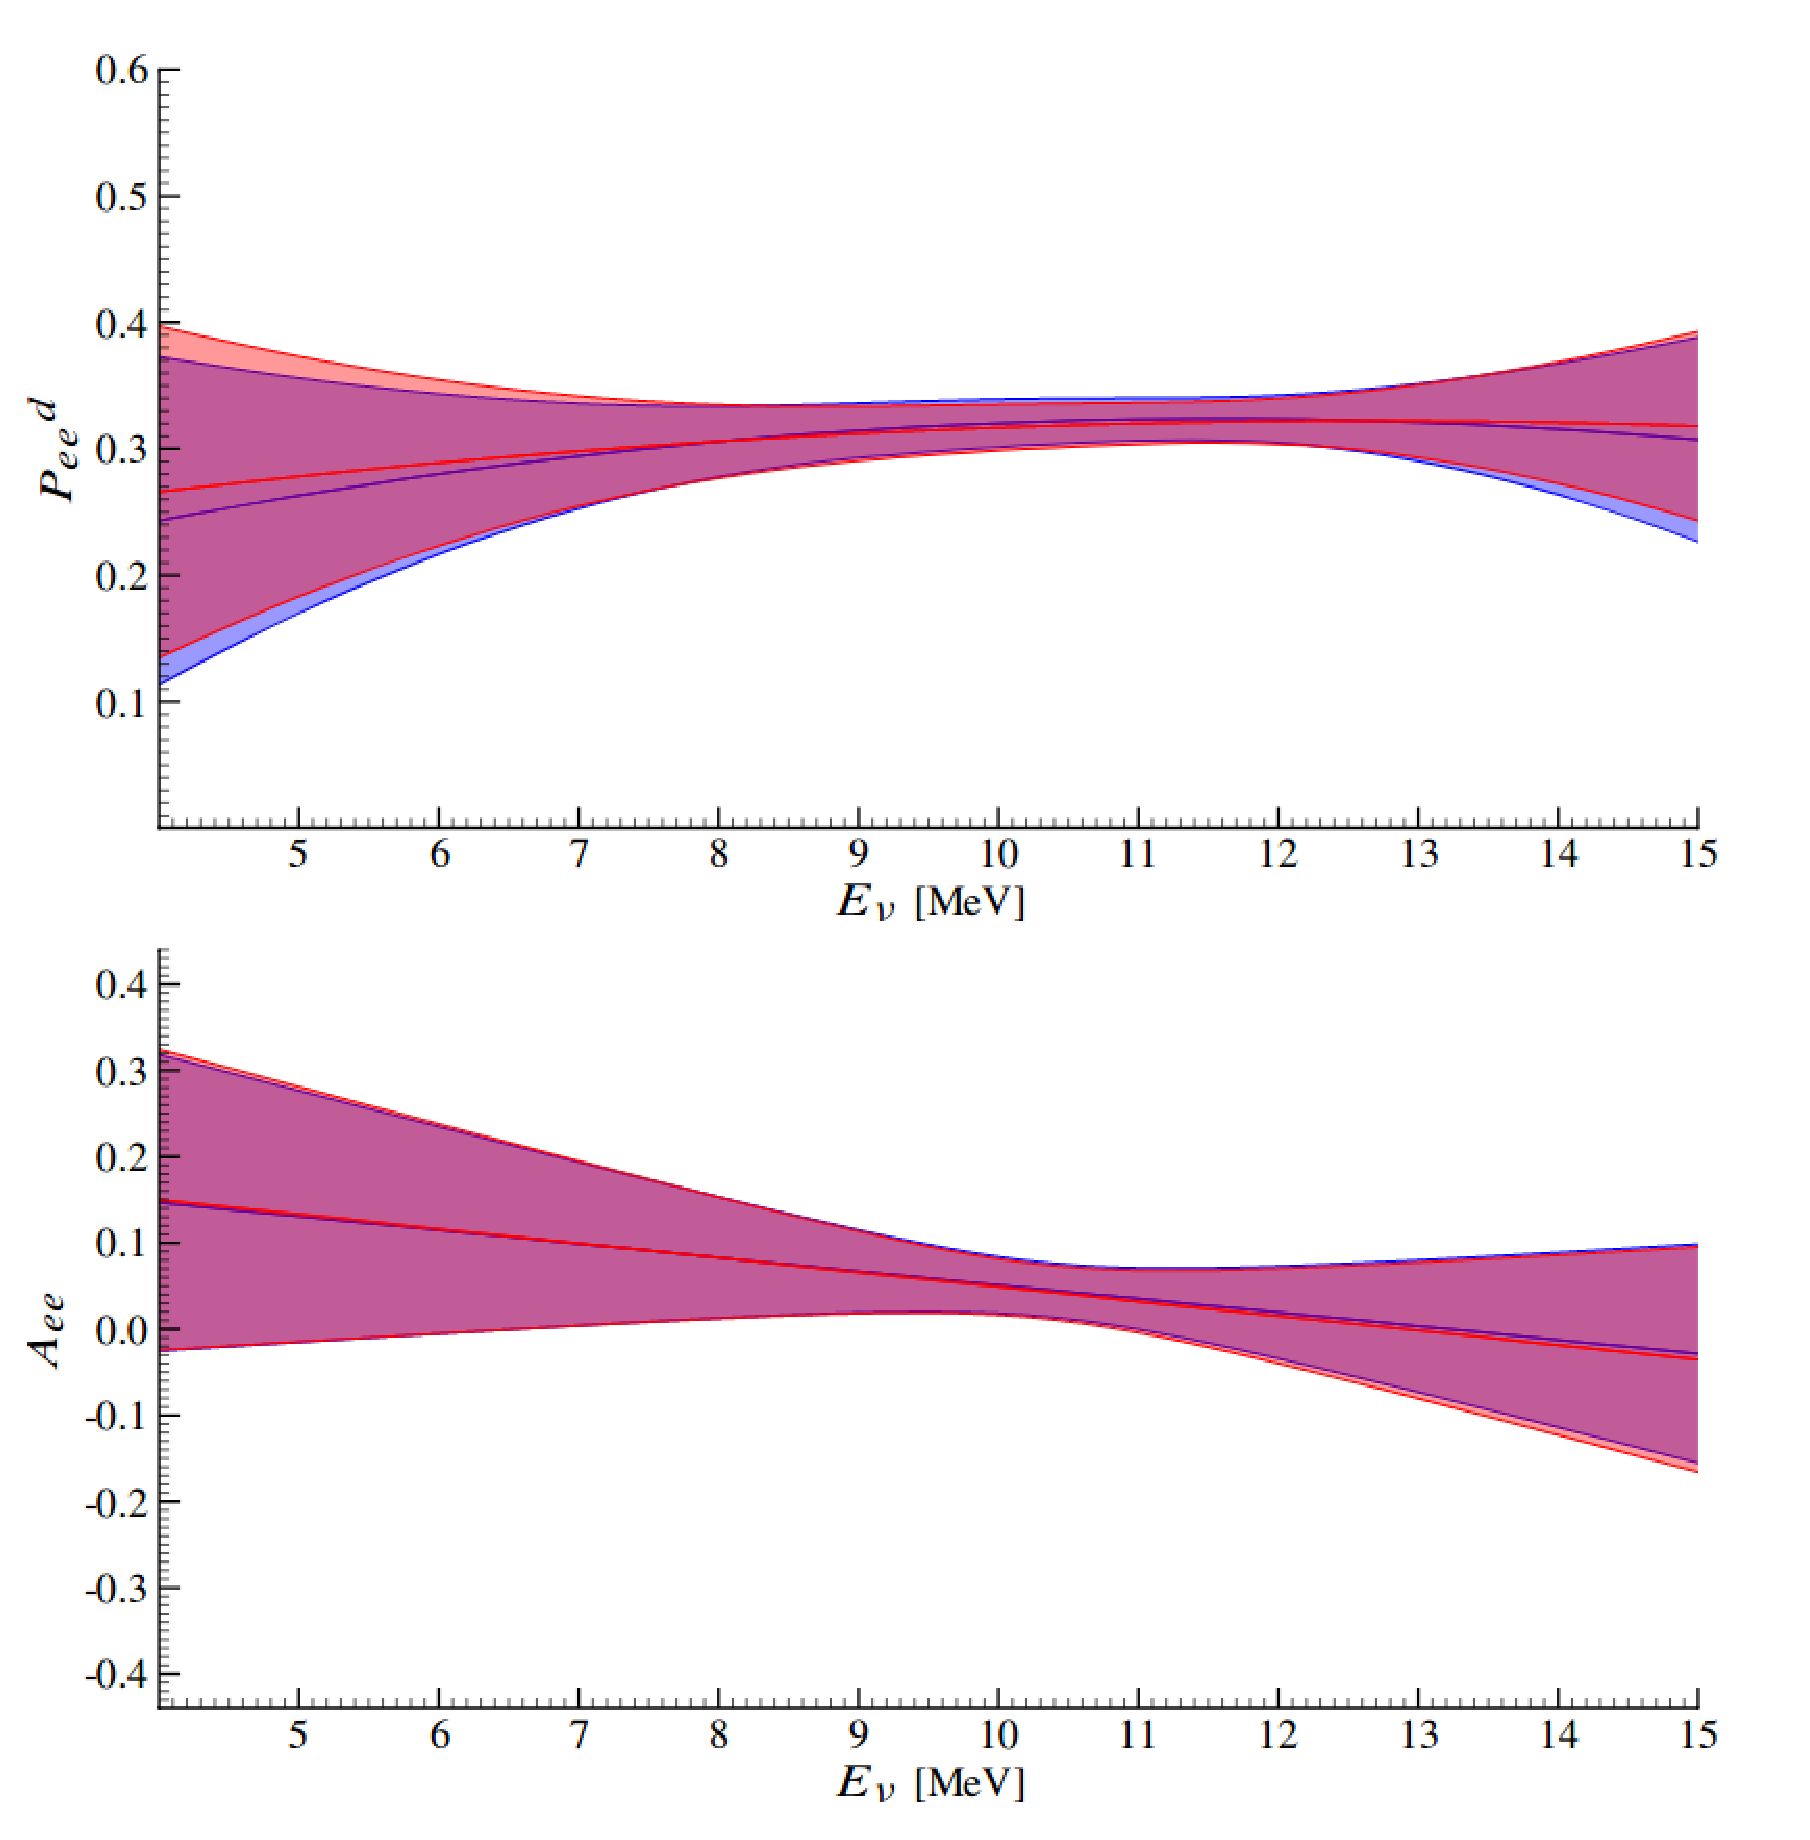
\includegraphics[width=\textwidth]{sno_pee}
        \caption[]{}
        \label{fig:sno_pee}
    \end{subfigure}
    \hfill
    \begin{subfigure}[b]{0.58\textwidth}
        \centering
    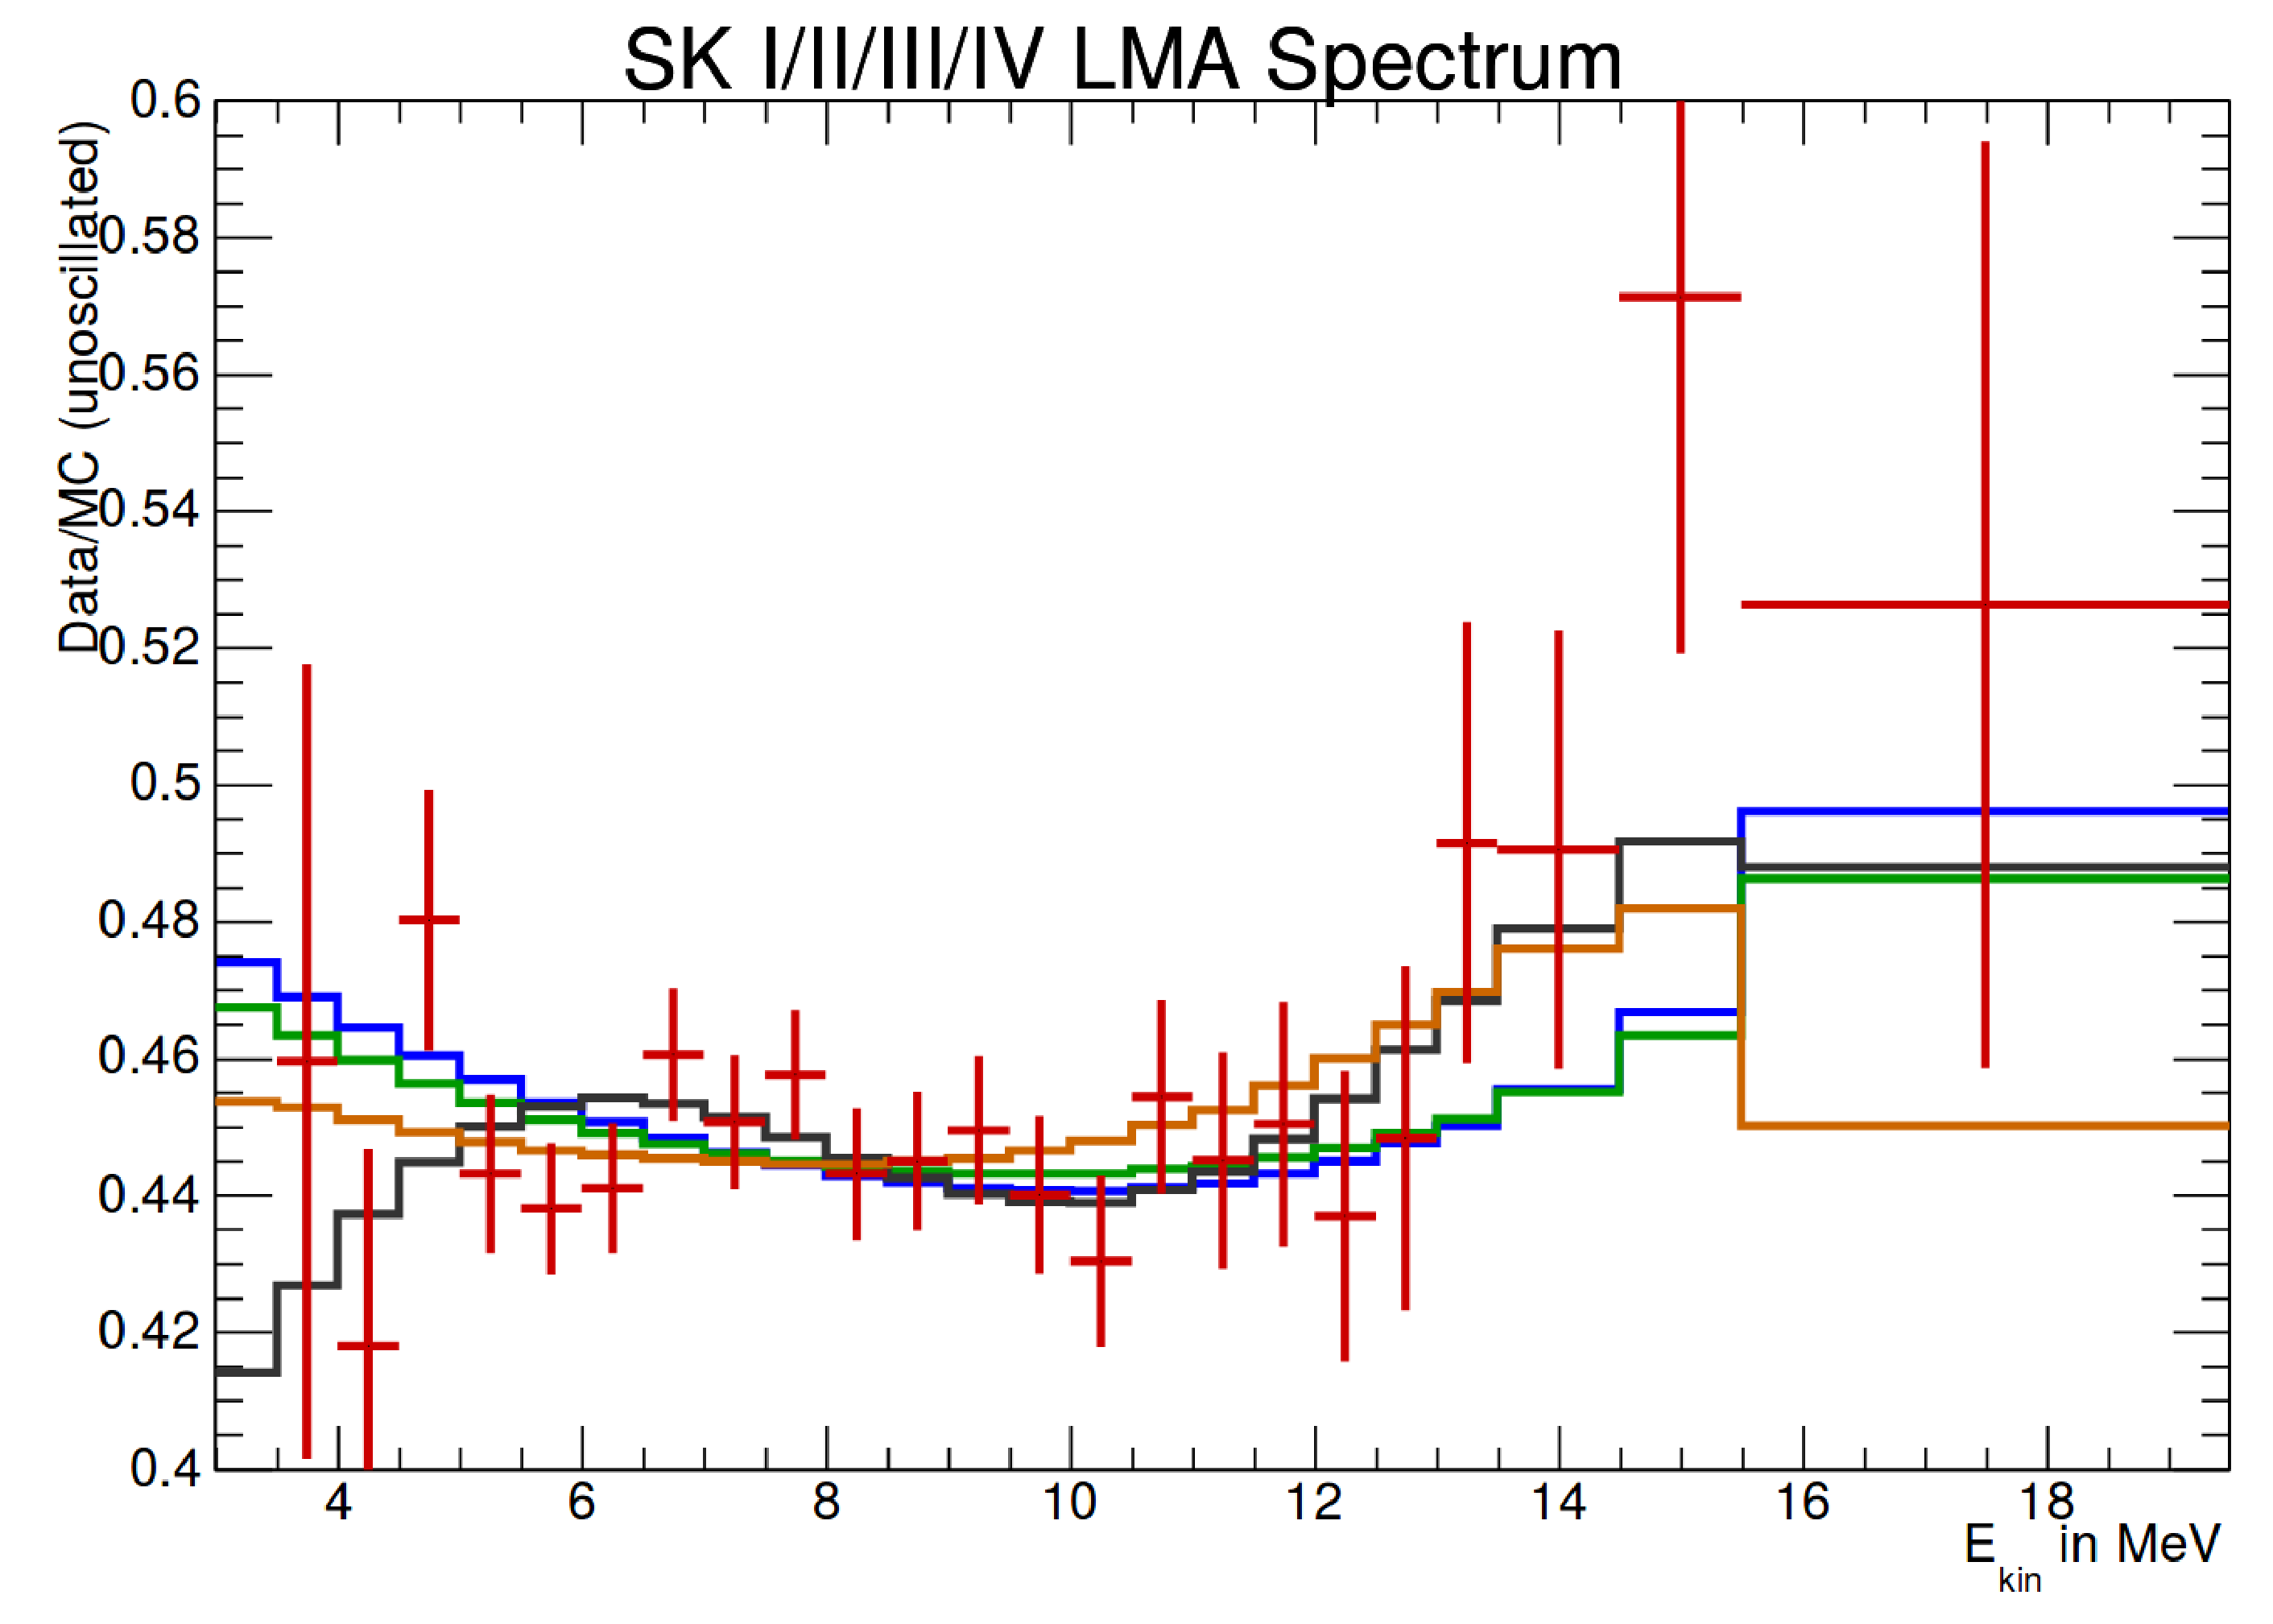
\includegraphics[width=\textwidth]{sk_spectrum}
        \caption[]{}
    \end{subfigure}
    \caption[]{}
    \label{fig:es_b8_measurement}
\end{figure}

Because the ``up-turn'' in the survival probability has not yet been observed,
solar neutrino measurements of $\Delta m^{2}_{21}$ prefer relatively low values
that push the transition region to lower energies.
Using only data from SNO and SuperK the best fit value for 
$\Delta m^{2}_{21}$ is
\begin{equation*}
    \Delta m^{2}_{21} = (4.8^{+1.5}_{-0.8})\times 10^{-5} eV^{2}\text{\citep{superk4}.}
\end{equation*}


In principal, the transition region could be probed as well by a precise
measurement of the survival probability from $pep$ or $\ce{^{7}Be}$ neutrinos.
$pep$ neutrinos are mono-energetic at $E_{\nu}$ = 1.4\,MeV,
this means they should have a survival probability of $53\%$ instead of the
vacuum survival probability of about $56\%$.
$\ce{^{7}Be}$ neutrinos are also mono-energetic at $0.861$\,MeV, providing
them with an expected survival probability of $54\%$.
A measured deviations of these survival probabilities from the expected
vacuum mixing value would provide a measurement of $\Delta m^{2}_{21}$.
But so far measuring these fluxes to that level of precision has not been
possible.
The current best measurement of these neutrino fluxes comes from the Borexino
collaboration~\citep{borexino_nature}, their results are show in Tbl.~\ref{tbl:borexino_results}.
\begin{table}
    \centering
    \begin{tabular} {c| c c}
        & Measured Survival Probability [\%]\\
        \hline
        $pp$ & $056.6 \pm  9.2$\\
        $\ce{^{7}Be}$ & $53.2\pm 5.4$ \\
        $pep$ & $42.8\pm11.4$ \\
    \end{tabular}
    \caption[Borexino Measured Low Energy Survival Probabilities]{
        Measured survival probabilities for low energy solar neutrinos
        from the Borexino experiment~\citep{borexino_nature}.}
    \label{tbl:borexino_results}
\end{table}

The day-night effect also provides sensitivity to $\Delta m^{2}_{21}$.
The smaller $\Delta m^{2}_{21}$ is, the lower the energy threshold is for
neutrinos to experience significant matter effects as they travel through the
Earth.
In practice the day-night effect has been difficult to measure due to
the statistics required to measure a few percent change on the survival
probability.
And so the majority of sensitivity to $\Delta m^{2}_{21}$ for solar neutrino
experiments comes from their ability to measure the transition region.
The day-night asymmetry in the survival probability is often parameterized by the value $A_{ee}$, a value
defined as,
\begin{equation}
    A_{ee}(E_\nu) = \frac{P_{\text{ee, day}}(E_\nu) - P_{\text{ee, night}}(E_\nu)}{P_{\text{ee, day}}(E_\nu) + P_{\text{ee, night}}(E_\nu)}\text{.}
\end{equation}
The SNO measurement of this asymmetry is shown in the bottom panel of~\ref{fig:sno_pee},
they're result is consistent with no asymmetry.
The SuperK measured value for the asymmetry in the observed interaction rate (as opposed to
the survival probability) is
\begin{equation*}
    A_{R_\nu, SK} = (-3.3 \pm 1.0(stat.)\pm 0.5(syst))\%\text{.} 
\end{equation*}
This value is inconsistent with the no asymmetry at the roughly two-sigma level.
The predicted value for this asymmetry for the best fit KamLAND $\Delta m^{2}_{21}$
is $-1.7\%$ the predicted value for the SuperK+SNO value of $\Delta m^{2}_{21}$ is
$-3.3\%$.
So with relatively small significance, the solar measurement of $\Delta m^{2}_{21}$ from the day-night effect
prefers a lower value than the KamLAND measurement.
Figure~\ref{fig:sk_daynight} shows the SuperK asymmetry measurement in the
observed interaction rate.

\begin{figure}[htbp]
    \centering
    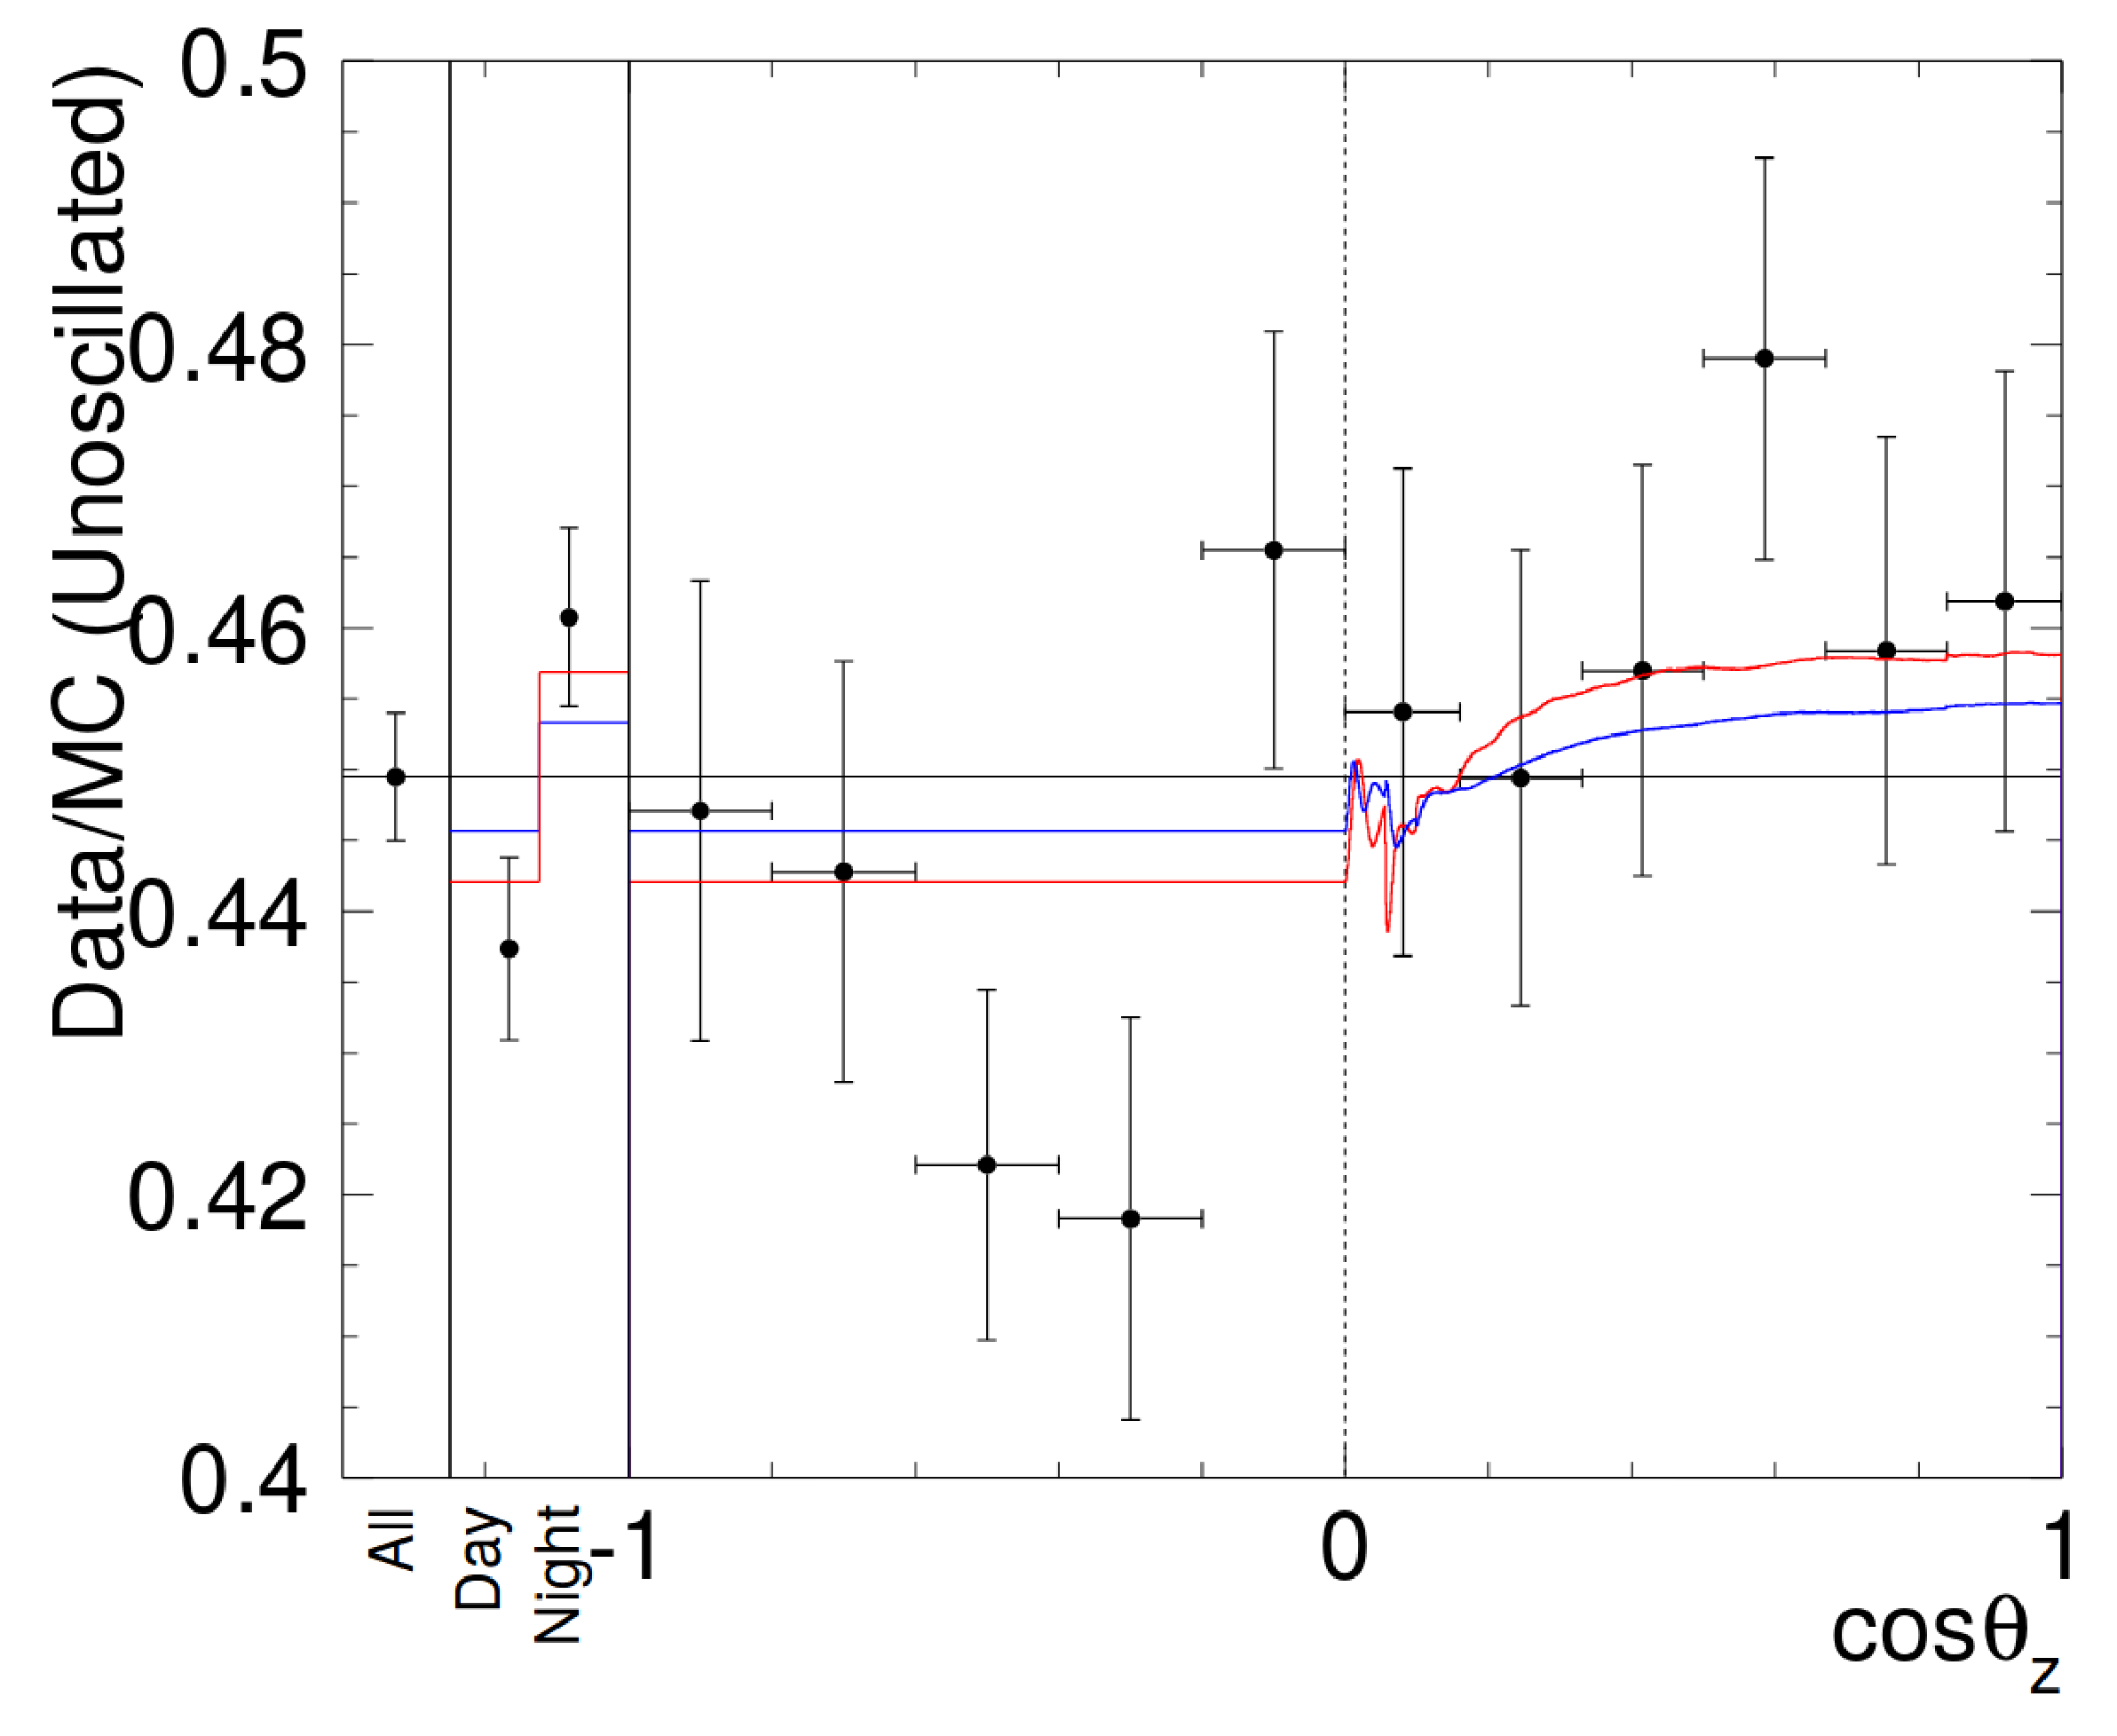
\includegraphics[width=0.78\textwidth]{sk_daynight}
    \caption[]{Figure from~\ref{superk4}}
    \label{fig:sk_daynight}
\end{figure}

Figure~\ref{fig:sk_pee_global} shows a summary of solar neutrino measurements
with the solar survival probabilities as predicted by the KamLAND+solar and
the solar only values for $\Delta m^{2}_{21}$.

\begin{figure}[htbp]
    \centering
    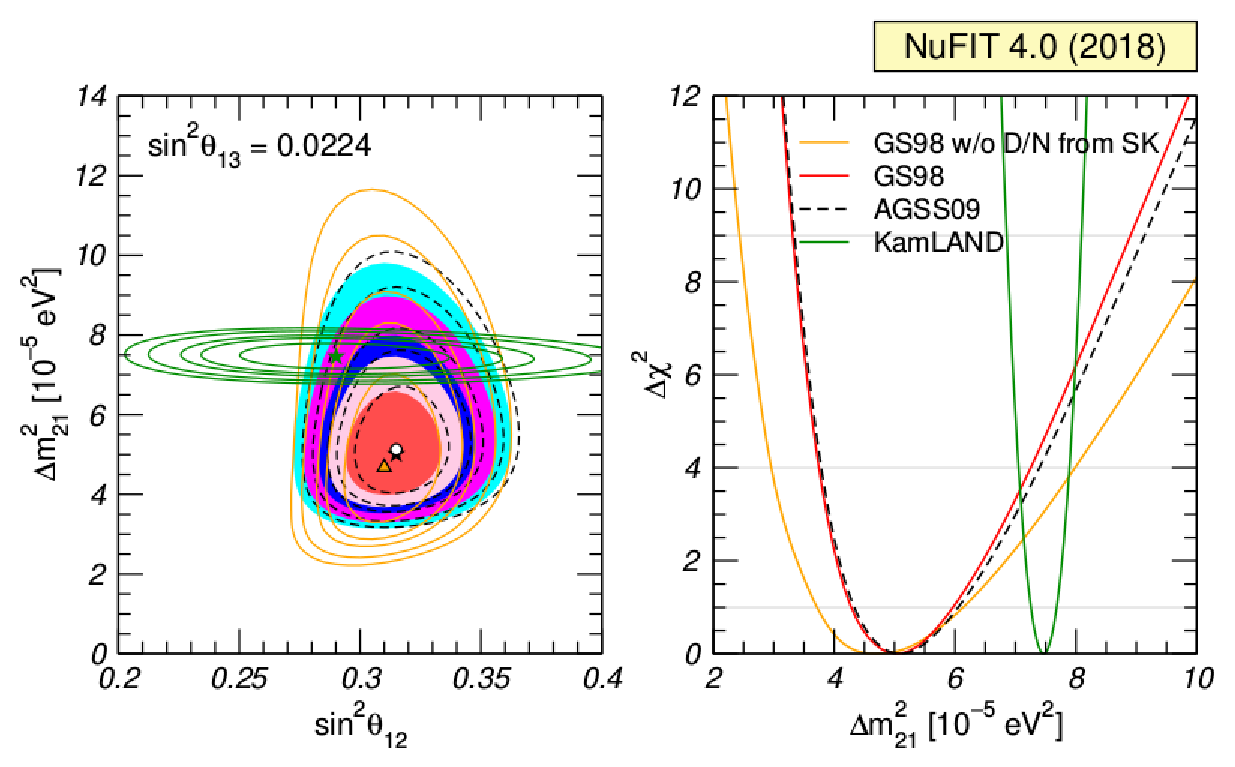
\includegraphics[width=0.78\textwidth]{nufit_dm21_tension}
    \caption[]{Figure from~\citep{nu_fit4}}
    \label{fig:nufit_dm21_tension}
\end{figure}
A global fit for solar neutrino parameters done by Esteban \textit{et. al.}~\citep{nu_fit4},
shown in Fig.~\ref{fig:nufit_dm21_tension},
the overall significance disagreement between the KamLAND+solar and the solar only
measurements for $\Delta m^{2}_{21}$.
They perform a fit to the solar data using solar model input from the GS98 solar abundances
as well as the AGS abundances, and show that uncertainty introduced by the
disagreement in those models is not sufficient to explain the consistently
low value for $\Delta m^{2}_{21}$ observed by SNO and SuperK.
They determine the disagreement between the solar and KamLAND values for
$\Delta m^{2}_{21}$ to have a significance of $\Delta \chi^{2} = 4.7$, or
roughly a $3\%$ chance of being the result of a statistical fluctuation.


\subsection{Non-Standard Interactions}
The observed discrepancy in the reactor and solar measured values for $\Delta m^{2}_{21}$
has motivated re-consideration of the models used to predict the solar survival
probability.
It's been shown that if neutrinos produced in the core of the Sun experience
significant flavor sensitive potentials their mixing could be sufficiently modified
to produce results consistent with the observed solar neutrino data, and
the KamLAND measured value for $\Delta m^{2}_{21}$~\citep{richie_nsi,mavans_nsi, nsi_friedland}.
Theories that modify the standard mixing model for neutrinos are generally
referred to as ``Non-Standard Interaction'' or NSI models, because
they often suppose the neutrino might couple to matter in some unexpected way.
Solar neutrinos provide an excellent laboratory for testing NSI models
because solar neutrinos are produced in and travel through matter densities much
higher than what is found in terrestrial neutrino experiments;
similarly solar neutrinos have a much longer baseline than any terrestrial
neutrino sources have.
Additionally, the neutrino production sources within the sun are well
relatively well understood and the Sun's density profile is also well
constrained by solar models.
These two factors allow for NSI theories to produce predictions for solar
neutrino observation that are precise but not ruled out by observations from
reactor, accelerator, or atmospheric neutrino experiments.

Beyond non-standard interactions there exist theories involving sterile neutrinos,
mass-varying neutrinos, neutrino decay, and large magnetic moments, all of
which modify the standard solar neutrino survival probability~\citep{maltoni_solar, richie_nsi}.
Figure~\ref{fig:maltoni_mixing} shows an example of survival probabilities
for a modified up and down quark neutrino interaction and a sterile neutrino
model.

\begin{figure}[htbp]
\centering
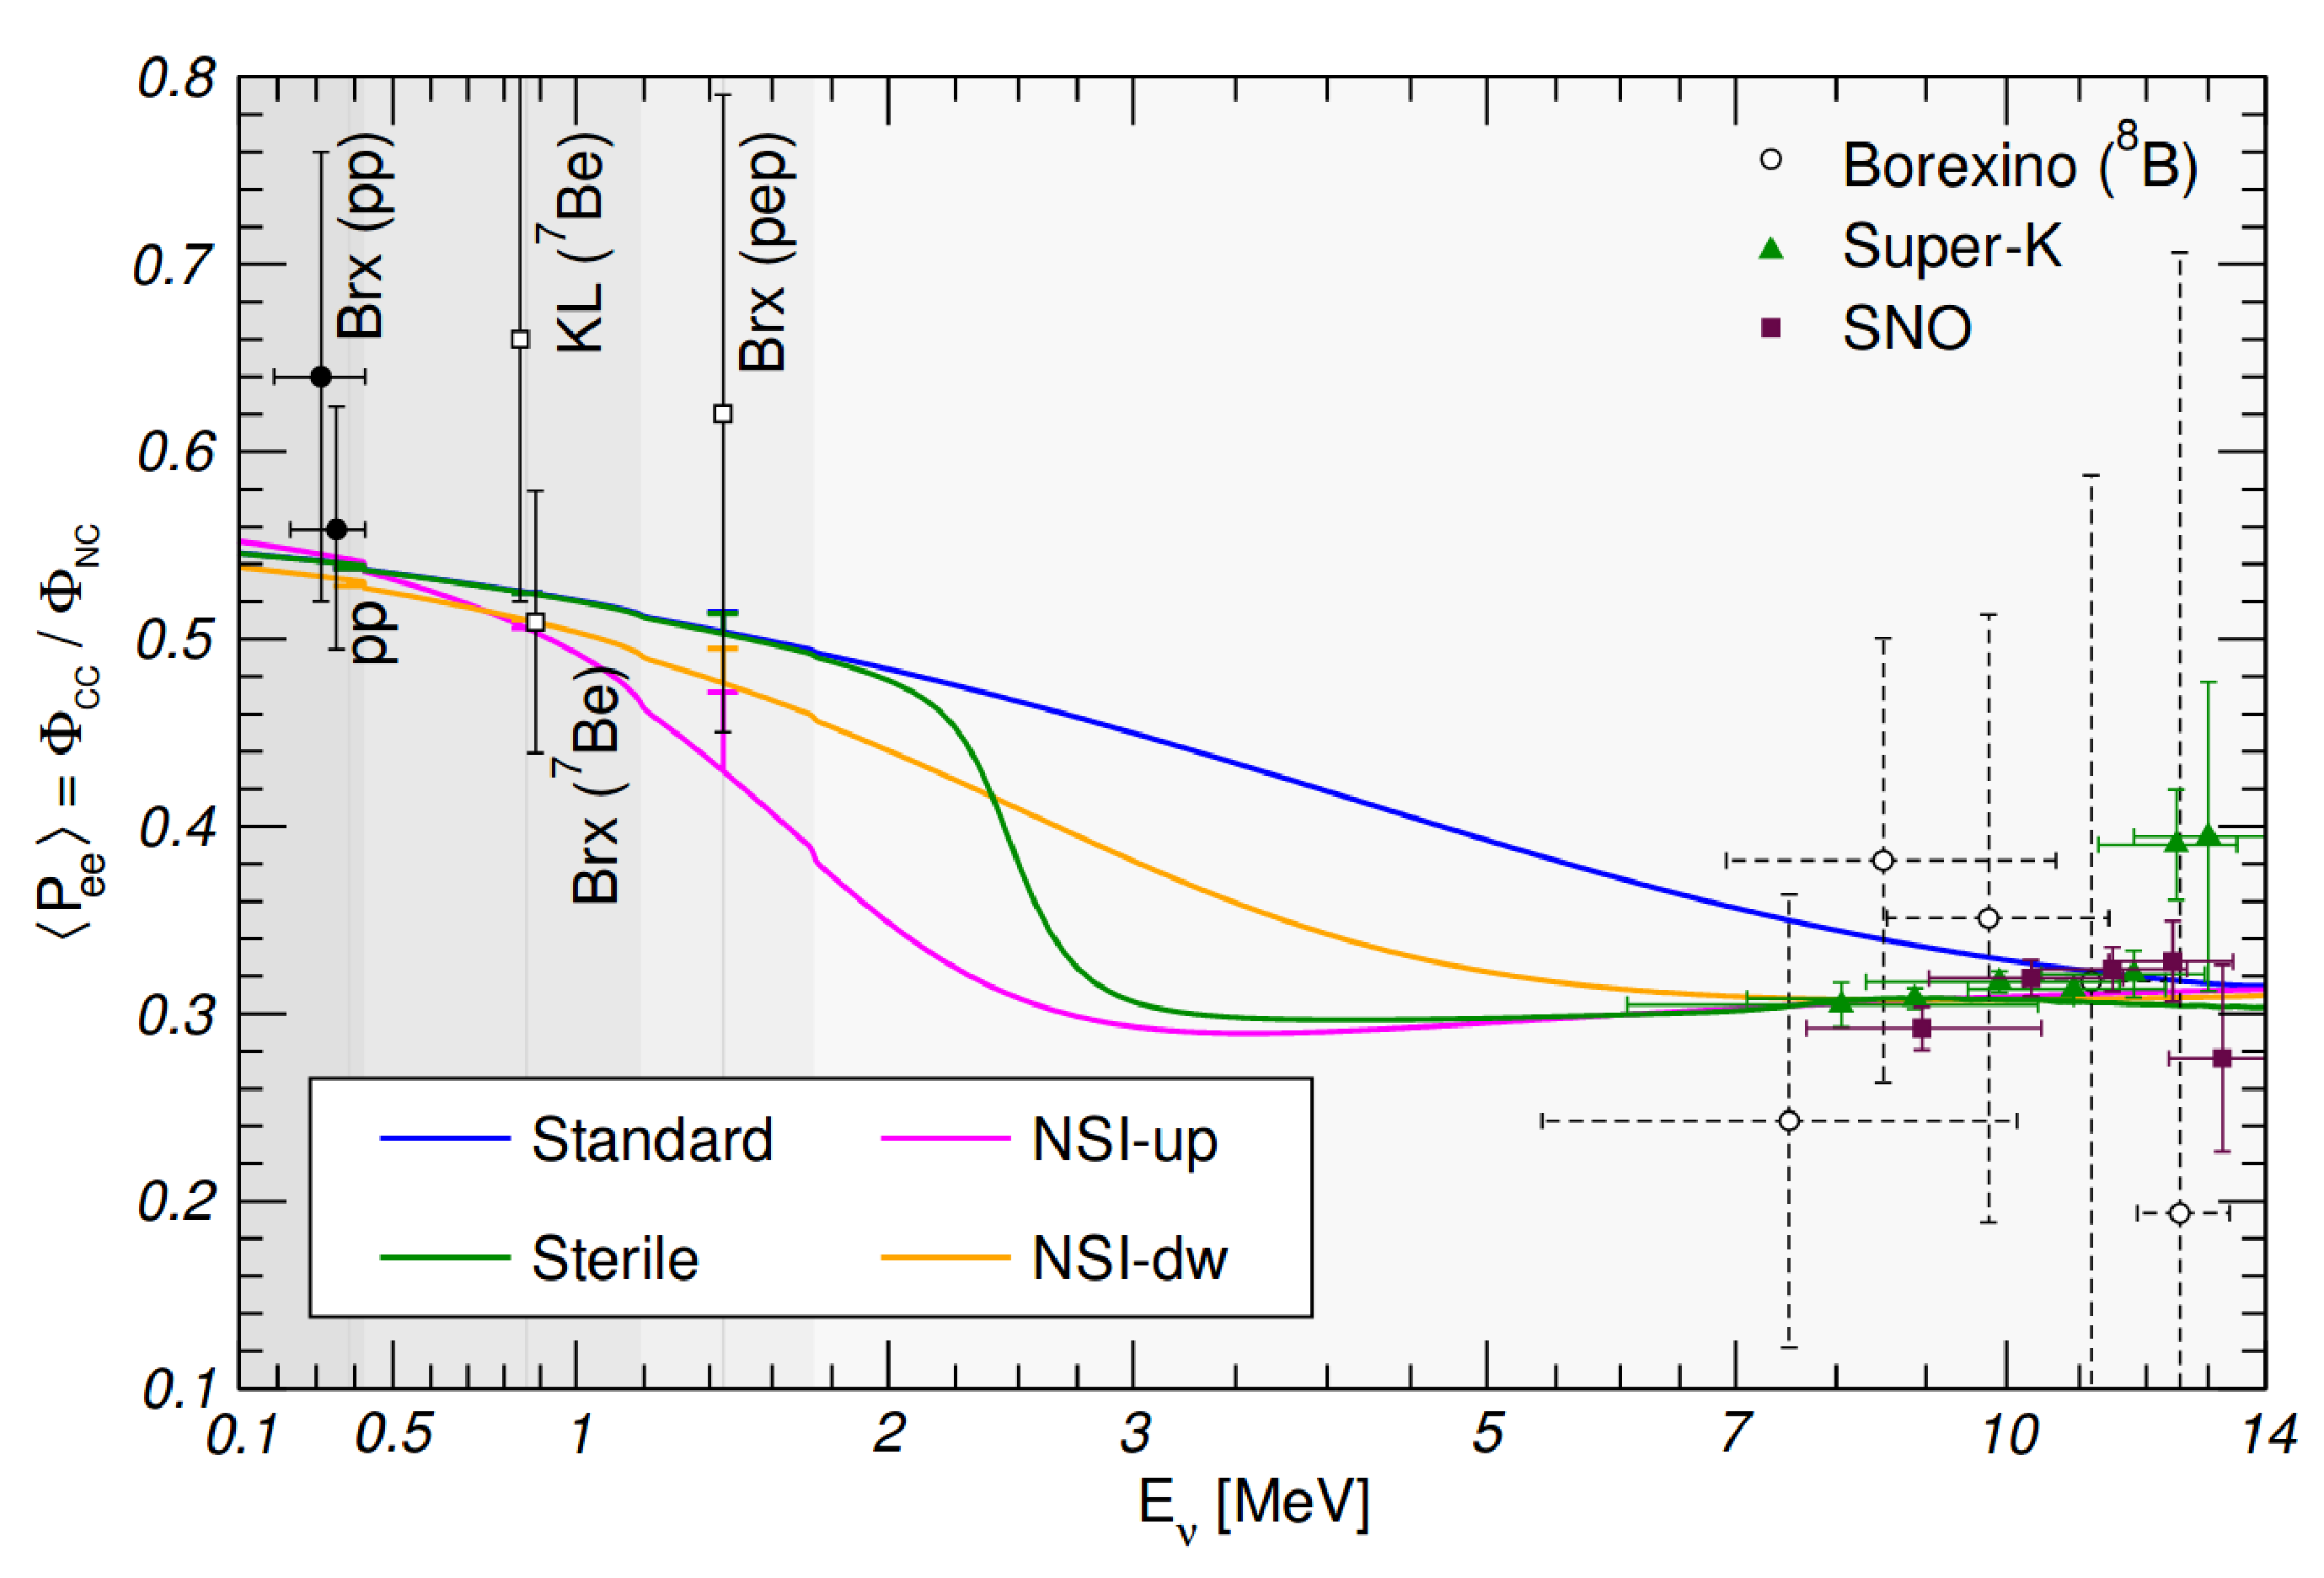
\includegraphics[width=0.78\textwidth]{maltoni_mixing}
\caption[]{Figure from~\citep{maltoni_solar}}
\label{fig:maltoni_mixing}
\end{figure}


\section{Modified Vacuum Mixing}
Considered here is a novel phenomenological theory that modifies the solar
neutrino survival probability.
Whereas many theories of modified neutrino mixing alter the way neutrinos
interact with matter, similar to standard matter enhanced-mixing,
here we consider a modification to neutrino mixing in areas of very low matter
density.
 Motivations for a potential with strength inversely related to local matter
density is considered in Sec.~\ref{sec:actual_chameleons}.
The effect A potential of this form is might have on neutrino
mixing is parameterized as follows
\begin{equation}
H = UM^{2}U^{\dagger} + A_{v}\text{,}
\end{equation}
where $U$ $M^{2}$ $A_{v}$ 





%\subsection{Chameleons}
%\label{sec:actual_chameleons
%It was proposed in~\citep{khoury_chameleons} that the observed expansion
%of the universe could be explained by introducing a 5th force that is weak
%in areas of high matter density. Such a force would be difficult to detect
%in most experiments because its effects would be small compared to standard
%forces. But at cosmological distance scales where the matter density is near
%zero, the force could be much stronger. This force is referred to as a ``chameleon''
%force, because it is affected by it's surrounding and can ``blend in'' to avoid
%detection.
%
%It could be the case that this force couples to neutrinos such that the coupling
%is sensitive to either neutrino flavor, or the mass. If so it's expected that the
%neutrino's mixing would be modified by the prescesce of a chameleon field.
%And that the chameleon-modified mixing would be only significant in areas of very
%low matter density.
%Solar neutrinos would provide almost unique sensitivity to this sort of modified
%vacuum mixing, because they're by far the most abundant and easily detectable source
%of neutrinos that travel a significant distance in areas of near-zero matter
%density, \textit{ i.e.}\ between the Sun and Earth.
%
%This idea is the phenomonlogical basis for the idea of modified vacuum mixing.
%To explore this idea I developed a simulation of neutrino mixing in the sun and in
%the vacuum. Typical calculations of the neutrino survival probability from
%the sun are able to take advantage of the fact that the neutrino travels adiabatically
%through the varying mass density of the sun. This means that the neutrino is
%created in a mixture of mass states, the exact composition depending on the local
%electron density, and the neutrino stays in that same mixture of mass states
%as it exits the sun. The flavor composition of each mass state however changes,
%meaning that the flavor composition of the neutrino state changes, even though
%it's mass-state composition does not.
%This means that practically all one needs to do is calculate the composition
%of mass states that corresponds to an electron type neutrino, and then calculate
%the flavor content of that composition in vacuum, and that flavor content
%tells you the survival probability and transition probability. One is able to
%ignore all oscillations that may occur within the sun and simply calculate
%quantities for when the neutrino is created and when it is detected.
%
%This simplification is not necessarily valid depending on how the neutrino
%exits the sun and how quickly the modified vacuum potential becomes significant.
%While the matter density is low but non-zero the neutrino will experience standard
%vaccuum mixing. If the neutrino changes from low to zero matter density over
%a distance much shorter than the oscillation length of the neutrino, the
%transition from standard to modified vacuum mixing potential may not be adiabatic.
%In which case the exact state of the neutrino at the point of the transition
%will determine how the flavor state of the neutrino changes as it propagates.
%
\section{Simulation}
Two different simulation of neutrino oscillations were developed, the first
does a full simulation of the neutrino state as it propagates from the
Sun to a detector at Earth.
Then second calculates the evolution
of the mixing eigenstates for solar neutrinos, and does not simulate individual
neutrinos.
The goal of both simulations is to produce a solar neutrino survival probability
for any given set of standard model mixing parameters and modified vacuum
mixing parameters.
These two simulations methods will be discusssed in greater detail in the following sections,
but the reason for the two different methods is to allow for different
trade-offs between detailed simulation and computational speed.

\subsection{Neutrino Simulation}
To allow for this the simulation for modified vacuum mixing simulates the full
neutrino state as it propagate through the sun. The equation
\begin{equation}
    \label{eqn:mixing_schrodinger}
    i\frac{d\Psi}{dx} = H\Psi %TODO
\end{equation}
is evaluated numerically using the Runge-Kutta method of numerical integration.
This cannot be easily evaluated analytically due to the varying density in the
core of the sun.
The electron density profile for the sun is given in XXX, and used to
estimate the matter potential at all points within the Sun.

Performing this simulation for many neutrino energies at many different starting
radii gives a representation of all possible neutrino states for solar neutrinos
as they exit the Sun. This ``library'' of possible solar neutrino states
is used as input to the modified vacuum potential simulation.

The standard solar survival probability can be calculated by calcuating
$|\bra{\nu_{e}}\ket{\Psi_{\nu}}|^{2}$ for each simulated neutrino and appropriatly
integrating over energies and production radii.
Since neutrino states are simulated by linearly sampling starting radii and logarithmically
sampling neutrino energies, states must be weighted by the relevant production
PDFs in energy and radius.
Figure~{XXX} shows the standard $\ce{^{8}B}$ survival probability simulated
this way.

The chameleon portion of the simulation is done by first monte-carlo sampling
neutrino energies and production radii, and looking up the simulated
neutrino state that corresponds to the sampled energy \& production radius.
The radial production PDFs for each neutrino type that are MC sampled from 
are given in~\citep{XXXradialproduction?}.
The neutrino energy PDFs are given by~\citep{BS05OP} and \citep{Winters},
however only half of all sample energies are drawn from the relevant prodcution
spectra, the other half are drawn from a uniform distribution from
0\,MeV to the relevant endpoint energy.
The motivation for this sampling method is discussed further at the end of
this section.
%This sampling method gurantees that no energy is so poorly sampled 
%that the simulation results are not useful, but also ensure that the most
%well sampled energies are those most typically produced in the Sun.

Since MC sampling produces energy and production radius values that fall
between bins used when producing the solar state library, the states
from the closest available radius bin is used. For energy
a random choice is made between the energy bins immediatly above and below
the desired energy is performed, the probability of choosing either bin
is dependent on how close the desired energy is to that bin.
This process is repeated for $1000000$ simulated neutrinos for each solar
neutrino type, \textit{e.g.} $\ce{^{8}B}$, $pep$, etc.

The simulation of neutrinos this way is computationally expensive. A few methods
were explored for ensuring this simulation could be performed in a reasonable
amount of time. The method that was used for nearly all of the results here was
to perform the Runge-Kutta integration on a GPU, which each thread corresponding
to a single sample in energy and production radius.

% TODO need typical radii/energy sample counts
However, even using GPU acceleration the simulation is still very time consuming,
a simulation of XXX energy samples and XXX production radius samples requires
roughly 2000\,gpu-hours. Performing this simulation as part of a fit to data would
require potentially hundreds or thousands of iteration. So it is not possible to
perform the full simulation in a fit.

Fortunately, by construction, the solar simulation is not effected by modified
vacuum potential; the main inputs to the solar simulation are the standard model
mixing parameters and the solar density profile. So, standard model mixing parameters
taken from KamLAND and other non-solar neutrino experiments can be used for
the solar simulation.

The result of the solar simulation is the neutrino state at 5000 samples
closest to the exit of the sun. Depending on the energy of the neutrino this
corresponds to state the neutrino is in in the final  150 to 500 km of
the Sun, this corresponds to \numrange{0.2}{0.7}\% of the solar radius ($R_{odot}$).
And the sample-to-sample distance is \numrange{30}{100} meters.
Production radii samples are XXX\,m from each other, meaning that
the \numrange{150}{500}\,km samples taken at the end of the simulation
overlap with samples taken one production radius step further.
This provides a useful check of the simulation, the difference between two
samples which have travelled the same distance within the sun should only depend
on the difference in electron density where they were produced.
Figure shows that correlation\ldots.%TODO!(maybe, not that important)

Once  monte-carlo samples of neutrino states produced by the Sun is calculated, these
states are used as inputs to a simulation of the modified vacuum potential.
This simulation is in principle the same as the solar simulation,
it simply involve evaluating Eqn.~\ref{eqn:mixing_schrodinger}, where $H$ now
corresponds to the modified vacuum Hamiltonian.
Unlike the solar simulation though the value of $H$ is not expected to change
as the neutrino propagates; Equation~\ref{eqn:mixing_schrodinger} can be evaluated analytically
between the Sun and Earth.

The final step of the calculation is to evolve the sampled neutrino states through
the Earth, to the detector.
This is done similarly to the simulation of neutrino propagation through the
Sun.
The calculation for this is done for only a ``day'' path through the earth
and a ``night'' path. The ``day'' path simulates the neutrino only travelling
through the crust of the Earth. The ``night'' path simulates the neutrino
travelling through the earth, including the high density ``core'' region.
a one-dimensional earth density profile is from~\citep{PREM} is used.
This results in an simulation of the day-night effect for neutrino
oscillation.

The result of this chain of simulation steps is monte-carlo samples
of neutrino flavor states. The survival probability is calculated as,
\begin{equation}
P_{ee}(\Psi_{nu}) = |\bra{\nu_{e}}\ket{\Psi_{nu}}|^2
\end{equation}
for each neutrino state.
Performing an average of survival probabilities binned neutrino energy 
gives the survival probability as a function of energy $P_{ee}(E_{\nu})$.

Since neutrino states are monte-carlo sampled to calculate $P_{ee}(E_{\nu})$
each value has statistical uncertainty from the number of samples used.
This problem was somewhat exacerbated by the distributions of some of the
solar neutrino energy PDFs having small values in areas that are important for
comparing to solar neutrino data. For example the low energy portion of the
$\ce{^{8}B}$ solar neutrino flux is very important for solar neutrino experiments,
but makes up a relatively small portion of the full $\ce{^{8}B}$ neutrino flux.
To mitigate the problem of large sampling uncertainty for important regions in
solar neutrino energy, energies were sampled according to a flat distribution
and according to the PDFs for each solar neutrino flux. These two methods of sampling
were performed in equal proportions for each flux type.

This method for calculating a modified vacuum survival probability has the
distinct drawback of being computationally expensive, to the point
where it cannot be used in a fit to data.
It does, however, have the benefit of simulating effects from a non-adiabatic
transition from between different potentials that effect neutrino mixing.
Non-adiabatic effects are important because the neutrino is neither produced nor
detected in a vacuum, so for modified vacuum potential to have an effect
that can be detected with a terrestrial detector there must be some
non-adiabatic transition.

\subsection{Neutrino Mass State Simulation} %TODO better subsection titles
The other method of simulation uses the same solar inputs as the
Runge-Kutta integration, but instead of simulating individiual neutrino
states, only the eigen-states are simulated.
For each production radius and production energy within the sun the
the mixing hamiltonian is diagonalized,
\begin{equation}
    H = U M U^{\dagger} + A = P D P^{\dagger}\text{.}
\end{equation}
Where $D$ is a diagonal matrix that gives the effective mass-squared
difference between the mass-states.
$P$ gives the flavor composition of the effective mass states,
$\ket{m_{1}}$, $\ket{m_{2}}$, $\ket{m_{3}}$.
The GNU Scientific Library~\citep{gsl_ref} is used to diagonlize
the mixing Hamiltonian.

A neutrino, produced in an electron flavor state, can be described as
\begin{equation}
    \ket{\nu} = \sum_{k=1}^{3}\braket{m_{k}}{\nu_{e}}\ket{m_{k}}\text{.}
\end{equation}.
The neutrino state is then evolved adiabatically into a modified
vacuum potential given by
\begin{equation}
    H = U M U^{\dagger} + A_{\mathrm{vac}}\text{.}
\end{equation}
The eigenstates from the modified vacuum Hamiltonian gives the neutrino mass
states $\ket{\mathrm{vac}_{1}}$, $\ket{\mathrm{vac}_{2}}$, $\ket{\mathrm{vac}_{3}}$.
So the neutrino state is now given by
\begin{equation}
    \ket{\nu} = \sum_{k=1}^{3}\braket{m_{k}}{\nu_{e}}\ket{\mathrm{vac}_{k}}\text{.}
\end{equation}
In general this equation could be used to evaluate the
survival probability, as is shown in Section~\ref{sec:neut_osc}.
However, equation~\ref{eqn:pee_adiabatic} shows that this process produces
terms that oscillate as the neutrino state evolves as well as constant
terms.
Solar neutrino experiments are not sensitive to oscillations in the survival
probability because the production of neutrinos is distributed
throughout the core of the Sun, which is many neutrino oscillation lengths
across.
For any detected neutrino
it's impossible to say where within the Sun the neutrino was produced.
Meaning there's no way to estimate how many oscillation lengths any neutrino
went through while traveling from the Sun to Earth, and so the oscillations
are effectively averaged over.

% TODO consider adding a wave-packet decoherence arguement here
%The second reason is that mass-states decohere while travelling from the Sun to Earth,
%meaning in a wave-packet treatment of neutrino oscillations the mass-states
%wave packets will have nearly zero overlap.

Because solar neutrino experiments are not sensitive to oscillations in
the survival probability allows for the survival probability to be calculated
by only the un-oscillating terms,
\begin{equation}
    P_{ee} = \sum_{k=1}^{3}\abs{\braket{m_{k}}{\nu_{e}}}^{2}\abs{\braket{\nu_{e}}{vac_{k}}^{2}}\text{.}
\end{equation}

This method for calculating the survival probability relies
on the neutrino entering the modified vacuum potential adiabatically.
Since the mechanism by which the neutrino is sensitive to the local matter
density is not considered here, it's plausible that the modified
vacuum potential ``turns-on'' slowly enough that there's no non-adiabatic
transition.
However, as mentioned earlier, since the solar neutrinos are neither
detected nor created in a vacuum, a non-adiabatic transition is required
for terrestrial neutrino detectors to be sensitive to a modified vacuum
neutrino potential.
For this model that non-adiabatic transition is assumed to be that the
neutrino does not fully transition from being best described
by a modified vacuum state by the time it's detected.
This is plausible because the oscillation length for higher
energy neutrinos is approximately 200\,km, the earth's atmosphere
is approximately the same size~\citep{atmosphere_profile}.
So it could be the case that solar neutrinos, especially at higher
energies, would not oscillate quickly enough to have a average
survival probability best described by the standard oscillation
probability.
For any set of mixing parameters this assumption can be checked using the
more computationally expensive neutrino state evolution simulation.

The benefit of this method for calculating modified vacuum solar survival
probabilities is that it's computationally much simpler and faster than the full
neutrino state evolution.
Allowing for a much wider amount of the parameter space for solar neutrino
mixing to be explored.

\section{Global Fit}
To determine solar neutrino and neutrino mixing parameters that is most
consistent with experimental observations, a fit is done to published
experimental results.
Solar neutrino results from SNO~\citep{sno_combined}, Super
Kamiokande~\citep{superk4, superk_first_solar,superk2, superk3},
Borexino~\citep{borexino_final_results,borexino_nature}, GNO~\citep{gallex, gno},
SAGE~\citep{sage}, and Homestake~\citep{homestake} are used.
Solar neutrino fluxes are constrainted by the GS98~\citep{gs98} solar abundance calculations.
Reactor neutrino results from Daya Bay~\citep{daya_bay}, KamLAND~\citep{kamland_reactor, kamland_data_release}, Reno~\citep{reno}
are also used to constrain neutrino mixing parameters.
The KamLAND experiment has also published solar neutrino
measurements~\citep{kamland_solar, kamland_b8},
only ther reactor neutrino results are used however.
Including the KamLAND solar results is a potential improvement for the global fitting
algorithm.
The KamLAND solar neutrino results are, however, compatible with and
significantly less constraining than the comparable measurements made by
Borexino, SNO and SuperK, so the inclusion of those measurements would not
effect any fit results significantly.

The software used for evaluating experimental consistency was developed
in part by Richard Bonventre~\citep{richie_thesis, richie_nsi},
but was updated to include more recent solar neutrino measurements
by the Borexino and Super Kamiokande experiments.
The software produces the likelihood of each experimental observation
for a given set of neutrino mixing parameter and solar neutrino fluxes.
Best fit parameters and uncertainties are found with the Minuit gradient
descent algorithm as well an MCMC algorithm. %TODO, probably just use one

The mixing parameters are primarily evaluated by producing a energy dependent
solar survival probability curve $P_{ee}(E_{\nu}$, then modifying the expected
solar neutrino event accordingly. %TODO, probably delete this sentence.


\subsection{Simplified Modified Vacuum Mixing}
Probing the idea of modified vacuum mixing with the simulation detailed in
section XXX proved computationally difficult.
So I explored simplified method for evaluating the likelihood of a modified
vacuum mixing potential. The simplification was to restrict the modified mixing
to be equivalent to a change in the effective value for $\Delta m^{2}_{21}$.
The motivation being that the observed discrepancy between solar neutrino
experiments and KamLAND was only in $\Delta m^{2}_{21}$, and not in $\theta_{12}$.

To explore this idea one simply can use standard methods for calculating the
survival probability, but modify them such that all terms are effected by the
local electron density ($n_{e}$) use a different value for $\Delta m^{2}_{21}$ than the
terms that are not effected by $n_{e}$.
This introduces a new parameter into the theory, $\Delta m^{2}_{21}\prime$, the
effective mass-squared splitting the neutrino experiences in vacuum.

With this modification a fit to solar neutrino data was performed, allowing
all mixing parameters to vary. If this version of modified vacuum mixing describes
reality then the best fit value for the matter mass-splitting ($\Delta m^{2}_{21}$) should be
consistent with the value determined by KamLAND.\@ The value for the vacuum mass
splitting ($\Delta m^{2}_{21}\prime$) has no-apriori preferred value but it would
be sensible for it to be near the standard best fit value for $\Delta m^{2}_{21}$
as determined by solar neutrino only measurements.

The fit to data was performed using a Markov-chain Monte-Carlo method to sample
the likelihood space of mixing parameters as well as solar neutrino fluxes.
Figure XXX shows the results of the MCMC sampling. Marginalizing over all
the mixing parameters, including $\Delta m^{2}_{21}\prime$, gives the best fit
value for $\Delta m^{2}_{21}$ in matter and the error on it.
The marginalized result is shown in Figure XXX, the preferred value
for $\Delta m^{2}_{21}$ from solar experiments is $XXX\pm XXX$, only slightly higher than
the preferred value in a standard mixing formulation, $XXX$, but still significantly
lower than the best fit KamLAND value, $XXX$.
The tension between the solar and KamLAND values of $\Delta m^{2}_{21}$ is at
the $XXX\sigma$ level in the standard formulation, this version of modified
vacuum mixing reduces that to $XXX\sigma$, at the cost of introducing a new
parameter into the theory.

The improvement in agreement between solar neutrino experiments and KamLAND on
the value of $\Delta m^{2}_{21}$ is not large enough to constitue compelling evidence
that this simple version of modified vacuum mixing describes reality much better
than standard mixing. And so this motivates going back to a fuller description
of modified vacuum mixing, that allows for a fuller description of how
neutrinos might oscillate between the Sun and Earth.
